\chapter{Lab File system:文件系统实验}
\begin{introduction}
    \item 使文件系统支持大文件
    \item 实现符号链接
    \item 现代的文件系统
\end{introduction}

文件系统作为操作系统的重要部分,在前面的实验中都没有涉及。因而,在本实验中,我们会深入改进 xv6 原先的文件系统,从而学习与文件系统相关的一些概念。

\section{使文件系统支持大文件}

在原始的 xv6 的实现中,其文件系统的部分与原版的 Unix v6 类似,均使用基于 inode 和目录的文件管理方式,但其 inode 仅为两级索引,共有 12 个直接索引块和 1 个间接索引块,间接索引块可以指向 256 个数据块,故而一个文件最多拥有 268 个数据块。我们需要将 xv6 的文件系统进行扩充,使之可以支持更大的文件。

xv6 的实验手册中推荐的方案是:使用三级索引,共有 11 个直接索引, 1 个间接索引块和 1 个 二级间接索引块,故总共支持文件大小为 $11 + 256 + 256 \times 256 = 65803$ 块。

首先我们修改 \lstinline{fs.h} 中的一些定义,使之符合三级索引的要求:
\begin{lstlisting}[language=C]
    #define NDIRECT 12
    #define NINDIRECT (BSIZE / sizeof(uint))
    #define MAXFILE (NDIRECT -1 + NINDIRECT + NINDIRECT * NINDIRECT)
\end{lstlisting}

由于文件的读写需要使用 \lstinline{bmap()} 来找到需要操作的文件块,故而我们修改 \lstinline{fs.c} 中用于找到文件块的 \lstinline{bmap()} ,使之能够支持三级索引。一个简单的思路是通过访问文件的位置来判断该位置是位于几级索引中,这样可以复用原先的大部分代码,而只需要实现二级间接索引的部分。笔者的实现如下:
\begin{lstlisting}[language=C]
static uint
bmap(struct inode *ip, uint bn)
{
  uint addr, *a;
  struct buf *bp;

  if(bn < NDIRECT - 1){
    if((addr = ip->addrs[bn]) == 0)
      ip->addrs[bn] = addr = balloc(ip->dev);
    return addr;
  }
  bn -= NDIRECT - 1;

  if(bn < NINDIRECT){
    // Load indirect block, allocating if necessary.
    if((addr = ip->addrs[NDIRECT - 1]) == 0)
      ip->addrs[NDIRECT - 1] = addr = balloc(ip->dev);
    bp = bread(ip->dev, addr);
    a = (uint*)bp->data;
    if((addr = a[bn]) == 0){
      a[bn] = addr = balloc(ip->dev);
      log_write(bp);
    }
    brelse(bp);
    return addr;
  }
  bn -= NINDIRECT;

  if(bn < NINDIRECT * NINDIRECT){
    uint dbr = bn / NINDIRECT;
    uint dbc = bn % NINDIRECT;
    if((addr = ip->addrs[NDIRECT]) == 0)
      ip->addrs[NDIRECT] = addr = balloc(ip->dev);
    
    bp = bread(ip->dev, addr);
    a = (uint*)bp->data;
    if((addr = a[dbr]) == 0){
      a[dbr] = addr = balloc(ip->dev);
      log_write(bp);
    }
    brelse(bp);

    bp = bread(ip->dev, addr);
    a = (uint*)bp->data;
    if((addr = a[dbc]) == 0){
      a[dbc] = addr = balloc(ip->dev);
      log_write(bp);
    }
    brelse(bp);
    return addr;
  }
  panic("bmap: out of range");
}
\end{lstlisting}

\begin{proposition}[使用 \lstinline{bmap} 的巧妙之处] 
    Unix 的文件系统中,将文件位置映射到块的位置的操作封装为 \lstinline{bmap()} 可谓十分经典的软件工程技巧。按照正常的实现思路,需要在读写函数中分别实现查找对应块的过程,而将该过程抽象出来单独处理,使得文件系统的实现更加灵活,且具有更好的可扩展性:因为若要更改文件系统的底层结构,读写的函数几乎无需更改,而只需改变文件块的查找规则即可。
\end{proposition}

此时 xv6 的文件系统应该能够支持上述的大文件,再次编译并运行 xv6 ,然后运行 \lstinline{bigfile} ,会得到类似下图的结果:
\begin{figure}[H]
  \centering
  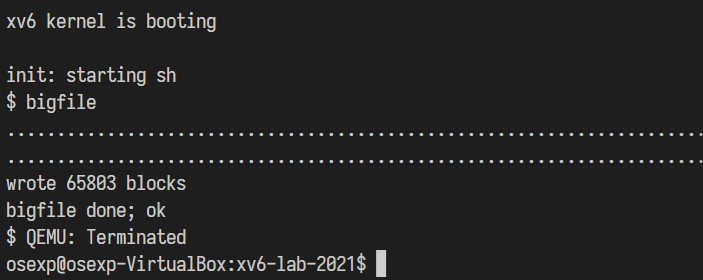
\includegraphics[width=0.8\textwidth]{fs_bigfile.jpg}
  \caption{ \lstinline{bigfile} 的测试结果}
\end{figure}

\section{实现符号链接}

在诸多类 Unix 系统中,为了方便文件管理,很多系统提供了符号链接的功能。符号链接(或软链接)是指通过路径名链接的文件; 当一个符号链接被打开时,内核会跟随链接指向被引用的文件。 符号链接类似于硬链接,但硬链接仅限于指向同一磁盘上的文件,而符号链接可以跨磁盘设备。我们需要实现一个系统调用 \lstinline{symlink(char *target, char *path)} 用于创建符号链接。

首先,按照通常的方法在 \lstinline{user/usys.pl} 和 \lstinline{user/user.h} 中加入该系统调用的入口,然后在 \lstinline{kernel/sysfile.c} 中加入空的 \lstinline{sys_symlink} 。修改头文件 \lstinline{kernel/stat.h} ,增加一个文件类型:
\begin{lstlisting}[language=C]
    #define T_SYMLINK 4   // Symbolic link
\end{lstlisting}

然后在头文件 \lstinline{kernel/fcntl.h} 加入一个标志位,供 \lstinline{open} 系统调用使用:
\begin{lstlisting}[language=C]
    #define O_NOFOLLOW  0x010
\end{lstlisting}

接着在 Makefile 中加入用户程序 \lstinline{symlinktest} ,此时应当能正常通过编译。这些准备工作完成后,我们可以真正着手实现 \lstinline{symlink(target, path)} 和对应的 \lstinline{open} 系统调用。在 \lstinline{sys_symlink} 中,仿照 \lstinline{sys_mknod} 的结构,创建节点并写入软链接的数据:
\begin{lstlisting}[language=C]
uint64 sys_symlink(void)
{
  char target[MAXPATH], path[MAXPATH];
  struct inode *ip;
  if(argstr(0, target, MAXPATH) < 0 || argstr(1, path, MAXPATH) < 0)
  {
    return -1;
  }
  begin_op();
  if((ip = namei(path)) == 0)
  {
    ip = create(path, T_SYMLINK, 0, 0);
    iunlock(ip);
  }
  ilock(ip);
  if(writei(ip, 0, (uint64)target, ip->size, MAXPATH) != MAXPATH)
  {
    return -1;
  }
  iunlockput(ip);
  end_op();
  return 0;
}
\end{lstlisting}

注意到其中调用了创建节点的函数 \lstinline{create} ,故我们也要对其进行修改:

然后修改 \lstinline{sys_open} ,使之能够跟随软链接并读取其指向的内容:
\begin{lstlisting}[language=C]
uint64
sys_open(void)
{
......
    if(ip->type == T_SYMLINK) 
    {
      if((omode & O_NOFOLLOW) == 0)
      {
        char target[MAXPATH];
        int recursive_depth = 0;
        while(1)
        {
          if(recursive_depth >= 10)
          {
	        iunlockput(ip);
	        end_op();
	        return -1;
	      }
          if(readi(ip, 0, (uint64)target, ip->size-MAXPATH, MAXPATH) != MAXPATH)
          {
	        return -1;
	      }
          iunlockput(ip);
	      if((ip = namei(target)) == 0)
          {
	        end_op();
	        return -1;
	      }
	      ilock(ip);
	      if(ip->type != T_SYMLINK)
          {
	      break;
	      }
	      recursive_depth++;
        }
      }
    }
......
\end{lstlisting}

至此,对于 xv6 的软链接功能已经完成,再次编译并运行 xv6 ,然后运行 \lstinline{symlinktest} ,会得到类似下图的结果:
\begin{figure}[H]
  \centering
  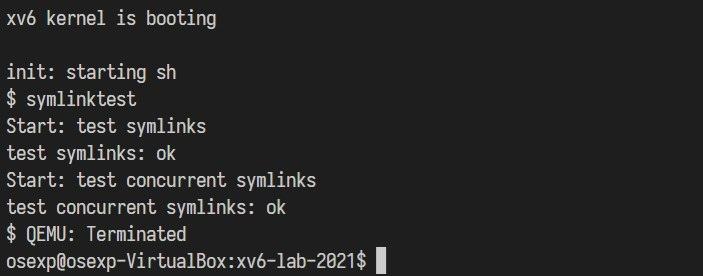
\includegraphics[width=0.8\textwidth]{fs_symlink.jpg}
  \caption{ \lstinline{symlinktest} 的测试结果}
\end{figure}

可见成功通过测试。

\paragraph*{实验结果} 在完成 Lab File system 中的所有实验后,根据 MIT 6.S081 的传统,需要在实验目录下创建一个名为 \lstinline{time.txt} 文本文件,其中只包含一行,为完成该实验的小时数。然后在终端中执行 \lstinline{make grade} ,即可对整个实验进行自动评分,笔者的结果如下:
\begin{figure}[H]
  \centering
  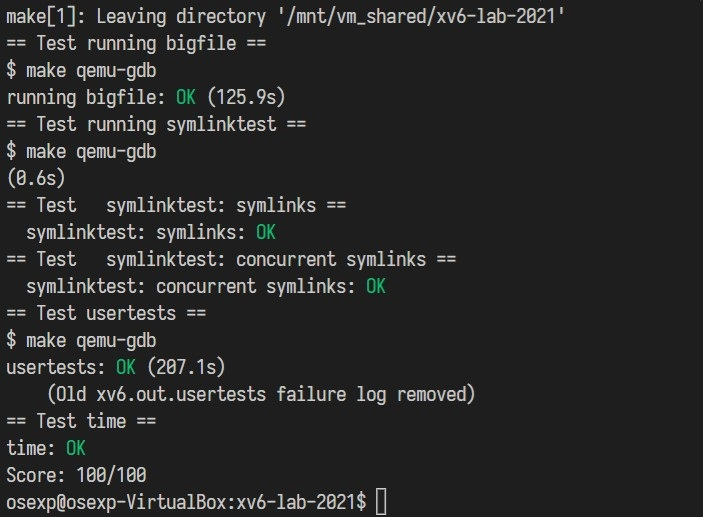
\includegraphics[width=0.8\textwidth]{fs_grade.jpg}
  \caption{ Lab File system 的测评结果}
\end{figure}

可见测试全部通过,得分为满分。

\begin{theorem}[注意 inode 加锁及其不同形态]
    在实现软链接的过程中,我们会碰到很多直接操作 inode 的情况。这些操作分布在不同的源文件中,有着复杂的加锁和写回机制,并且有着严格的执行条件。为了理清这些操作,需要理解 inode 、 inode 在内存中的映像和物理块等概念,并且仔细阅读各个函数前的说明:它们会提示我们该函数对目前加锁情况的要求,以及在函数完成后加锁情况的变化。
\end{theorem}
\section{小结:现代的文件系统}

在这个实验中,我们已经涉及了 Unix 文件系统的很多特性,且被我们完善过的 xv6 文件系统已经与一些较早的现代文件系统(如 ext2 )几乎一致,包括了如下的特性:
\begin{enumerate}
    \item 基于 inode 的多级索引文件组织
    \item 日志文件系统
    \item 硬链接和软链接
    \item inode 缓存与数据块缓存
    \item 基于缓存的写入优化
\end{enumerate}

但是,在上面的实验中,仍有一些现代文件系统的特性在 xv6 中没有被涉及,这里小结如下:
\begin{enumerate}
    \item 基于 Extent 的空间管理方式
    \item 成组的空间管理
    \item 基于 B 树的索引
    \item 原子性读写操作
    \item 跨物理卷管理
    \item 软件 Raid 机制
    \item 快照机制
    \item 只读文件系统优化
\end{enumerate}

上面一些机制在目前的一些文件系统中有着广泛的应用,就笔者的个人观点,参考学习 ext4 、 xfs 、 btrfs 、 erofs 这几个极具代表性的现代文件系统,便可以对上述特性的原理与实现有所了解,并且把握操作系统中文件系统的发展方向。